% little trick to replace lib.tex by this
\renewcommand{\doctitle}[1]{
	\chapter{#1}
}
\renewcommand{\biblio}[1]{}
\doctitle{L'oscillateur contrôlé en tension (VCO)}
\subsection{Fonctionnement et théorie}
La figure \ref{fig:schema_bloc_vco} nous montre le schéma bloc du VCO.
\begin{figure}[ht]
	\centering
	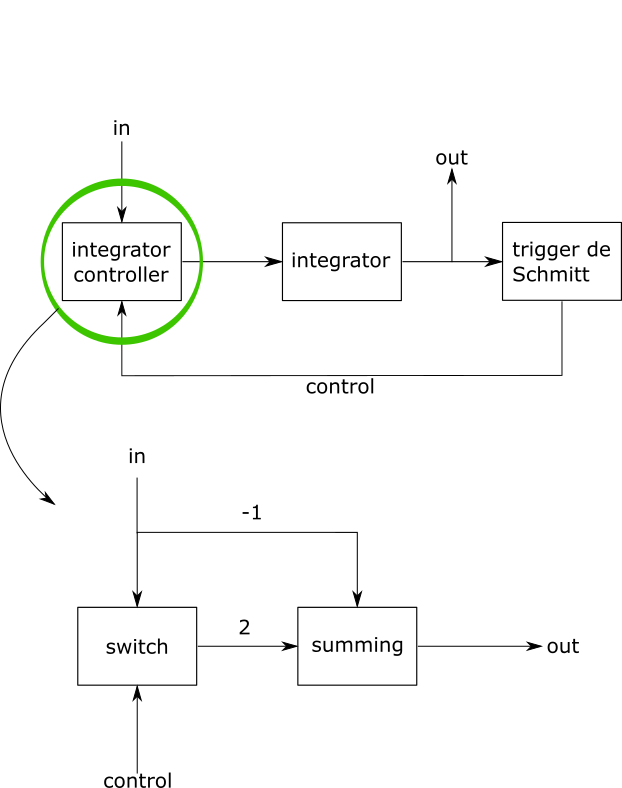
\includegraphics[width=0.4\textwidth]{img/schema_bloc_vco.png}
	\caption{Schéma bloc du VCO}
	\label{fig:schema_bloc_vco}
\end{figure}
Le VCO se compose des 3 blocs suivants:
\begin{itemize}
\item l'integrator controller (le contrôleur de l'intégrateur) qui se compose lui-même d'un switch et d'un summing (sommateur)
\item l'integrator (intégrateur)
\item le trigger de Schmitt (bascule à hystérèse)
\end{itemize}

Le signal d'entrée ($in$) est constant et vaut $\alpha$. Appelons $V_L$ la tension de basculement inférieure du trigger, $V_H$ la tension de basculement supérieure et $V_{CC}$ la tension d'alimentation du trigger.
Si la sortie du trigger de Schmitt ($control$) vaut $0$, la sortie du switch de l'integrator controller vaut $0$. Dès lors, la sortie du bloc integrator controller vaut $-\alpha$.  Après passage dans l'integrator, nous avons la droite $-K\alpha t$ avec $K$ la constante de temps de l'integrator. La sortie du trigger restera à $0$ tant que la sortie de l'integrator est supérieure à $V_L$. Lorsque la sortie de l'integrator a atteint $V_L$, le trigger bascule et sa tension de sortie devient $V_{CC}$. Le switch change d'état et sa sortie devient $\alpha$. La sortie de l'integrator controller devient donc $\alpha$. Après passage dans l'integrator, nous avons la droite $K\alpha t$. La sortie du trigger restera à $V_{CC}$ tant que la sortie de l'integrator est inférieure à $V_H$. Lorsque la sortie de l'integrator a atteint $V_H$, le trigger bascule et sa tension de sortie devient $0$. Le switch rechange d'état et sa sortie devient $0$. Et nous pouvons recommencer la même boucle temporelle.

La fréquence générée par le VCO pour une tension d'entrée donnée ($\alpha$) s'exprime en fonction de $K$ et de $\Delta V = \vert V_H - V_L\vert $ par la relation suivante $$ f = \frac{K\alpha}{2\Delta V}$$

\subsection{Dimensionnement et circuit réel}
\paragraph{Circuit réel}
%image circuit
Sur la figure \ref{fig:circuit_vco} se trouve l'implémentation électronique du VCO décrit ci-dessus.
\begin{figure}[ht]
\centering
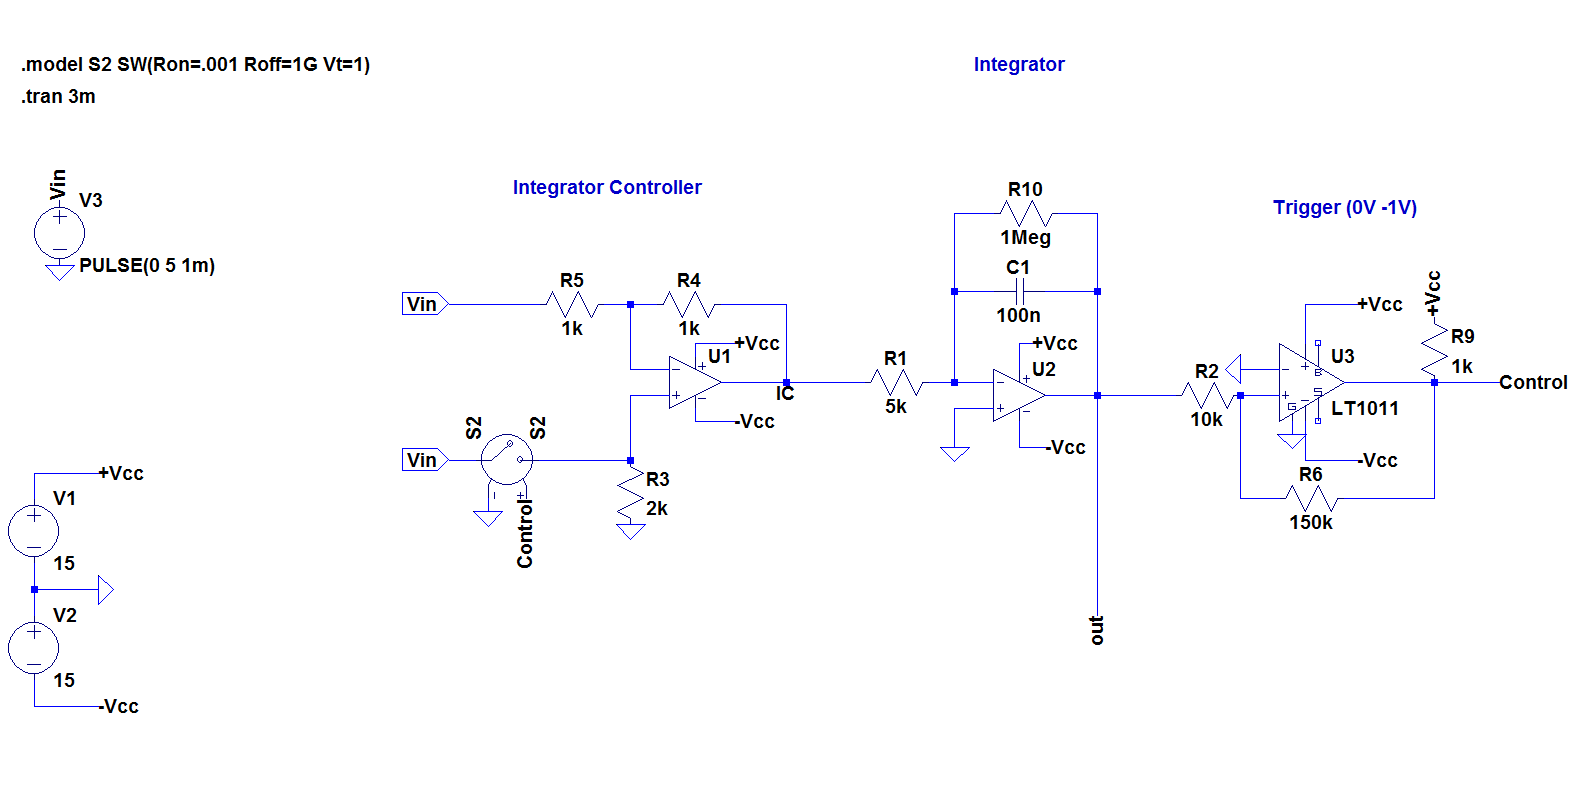
\includegraphics[width=16cm]{img/vco_circuit}
\caption{Circuit du VCO}
\label{fig:circuit_vco}
\end{figure}
\paragraph{Dimensionnement du trigger de Schmitt}
Le choix de placer le seuil supérieur ($V_H$) à \unit{0}{\volt} et le seuil inférieur ($V_L$) à \unit{-1}{\volt} est arbitraire. Cependant, la différence entre $V_H$ et $V_L$ doit rester au-dessus de \unit{500}{\milli\volt} pour éviter une influence des tensions parasites. Dans ce circuit, un trigger asymétrique est utilisé. Dès lors, le rapport des résistances à utiliser se déduit des formules suivantes : 
$$V_H=V_{REF}\left(1+\frac{R_2}{R_6}\right) \textmd{ et } V_L=V_{REF} + \frac{R_2}{R_6}\left(V_{REF}-V_{CC}\right)$$
Dans le montage du trigger asymétrique utilisé, $V_{REF}$, la tension à l'entrée non-inverseuse du comparateur vaut \unit{0}{\volt}. Dès lors, $\frac{R_2}{R_6}=\frac{1}{15}$
avec la condition que $R_6>>R_9$. Les valeurs de résistances choisies sont :
\begin{itemize}
\item \unit{10}{\kilo\ohm} pour $R_2$
\item \unit{150}{\kilo\ohm} pour $R_6$.
\end{itemize}

\paragraph{Dimensionnement de l'integrator}
Calculons maintenant la constante ($K$) du bloc integrator. Le VCO doit satisfaire la relation tension fréquence suivante : \unit{1}{\milli\volt} par \unit{}{\hertz}. Si la tension d'entrée est de \unit{1}{\milli\volt}, la fréquence de sortie est de \unit{1}{\hertz}. Comme le signal de sortie est un signal triangulaire, le temps de montée et de descente est identique. Le temps de montée vaut donc $\frac{1}{2*1} =  \unit{0,5}{\second}$. La pente de montée de la droite est de \unit{1}{\milli\volt}/\unit{}{\second}. Le temps pour monter ou descendre de \unit{1}{\volt} est de \unit{1000}{\second}. Comme il doit valoir \unit{0,5}{\second}, la constante d'intégration vaut 2000. D'où $\frac{1}{R_1C_1}=2000$ avec $C_1= \unit{100}{\nano\farad}$, $R_1 = \unit{5}{\kilo\ohm}$.
\paragraph{Dimensionnement de l'integrator controller}
L'integrator controller est constitué d'un ampli op en mode différentiel et d'un switch. L'équation constitutive de ce bloc est : $V_{IC}=2*V_+ - V_-$ avec $V_+$ la tension à l'entrée non-inverseuse et $V_-$, la tension à l'entrée inverseuse. La formule suivante permettant de déterminer une relation entre les résistances est obtenue en appliquant KCL : $$V_{IC}=V_+ \left(\frac{\left(R_4 + R_5\right)R_3}{R_3R_5}\right)-V_-\left(\frac{R_4}{R_5}\right)$$ Cela nous donne donc $R_5 = R_4 = 2R_3$.
Fixons $R_5$ à \unit{1}{\kilo\ohm}. Alors $R_4$ vaut \unit{1}{\kilo\ohm} et $R_3$ qui vaut \unit{2}{\kilo\ohm}.

\subsection{Confrontation  des mesures et de la théorie}
%TODO
\begin{figure}[ht]
	\centering
	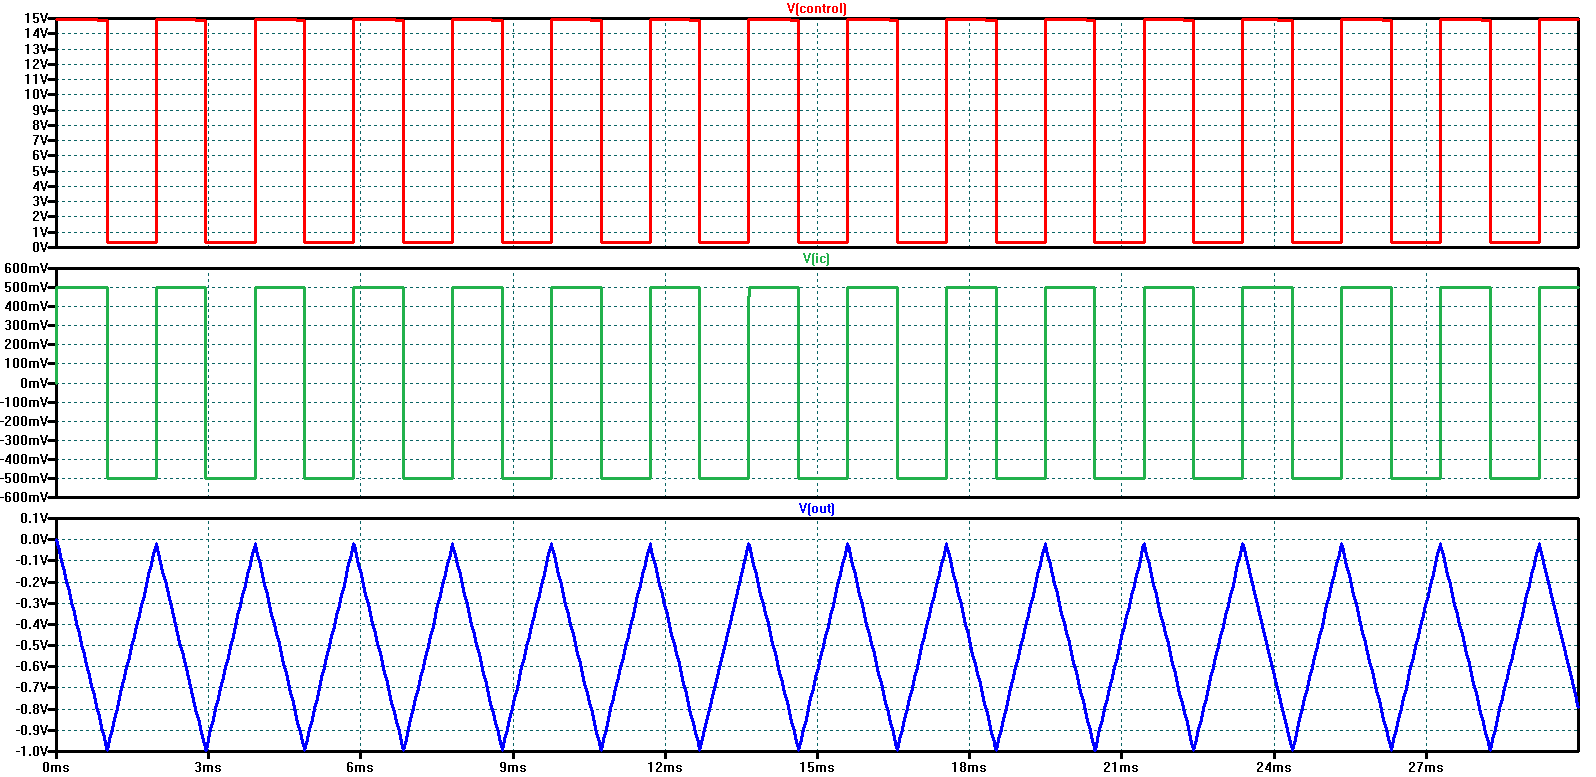
\includegraphics[width=0.8\textwidth]{img/vco_response.png}
	\caption{Simulation des signaux de sortie des différents blocs}
	\label{fig:out_vco_th}
\end{figure}
La figure \ref{fig:out_vco_th} affiche la simulation des signaux aux sorties des trois blocs fonctionnels pour une tension d'entrée de \unit{500}{\milli\volt}. Le signal à la sortie de l'integrator controller est affiché en vert et le signal à la sortie du bloc intégrator en bleu. Ce signal est également le signal de sortie finale du VCO. Pour terminer, le signal à la sortie du trigger est affiché en rouge.

\begin{figure}[ht]                                       
	\centering
	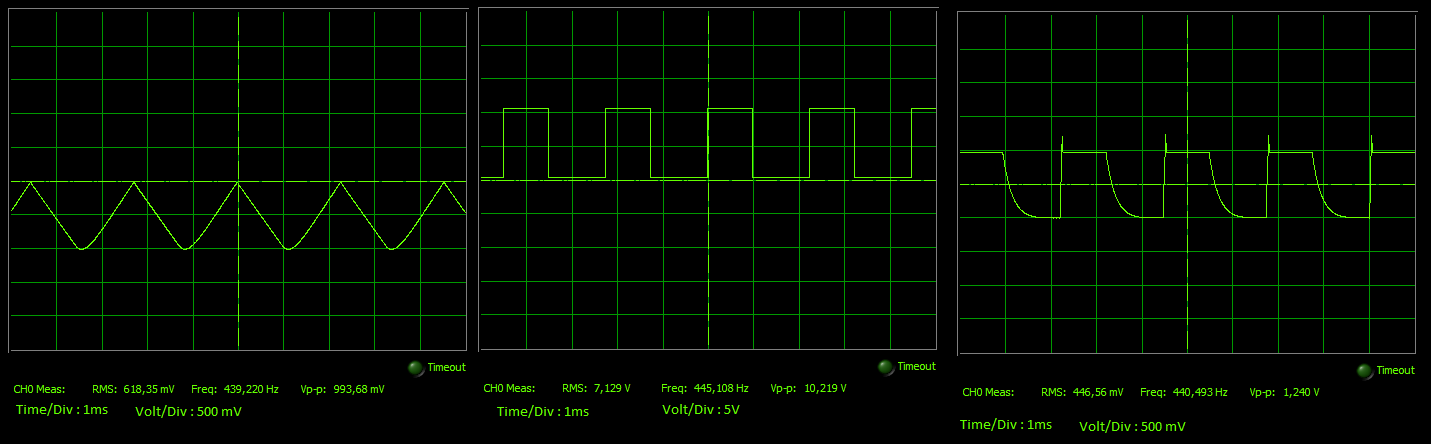
\includegraphics[width=0.8\textwidth]{img/vco_real_out.png}
	\caption{Sortie des différens blocs. De gauche à droite. Sortie de l'integrator, sortie du trigger et sortie de l'integrator controller}
	\label{fig:out_vco_real}
\end{figure}
La figure \ref{fig:out_vco_real} montre ces mêmes signaux aux sorties de circuit réel pour une tension d'entrée de \unit{500}{\milli\volt}. Les différences entre les deux sont très faibles excepté la sortie du bloc integrator controller qui en descente ne passe pas directement de on à off mais le fait progressivement. Cela ressemble à un effet capacitif au niveau du switch. Si la fréquence augmente, cet effet modifie complètement la réponse en fréquence du VCO.

%La figure \ref{fig:theory_vs_mesure} montre que la réalité est la théorie sont très proche. Les différences observées sont dues à des imprécisions des valeurs des résistances et des capacités. Cela provient aussi du switch qui contrairement au modèle utilisé dans les simulations et les calculs possède une légère courbe d'hystérèse.
%\begin{figure}
%	\centering
%	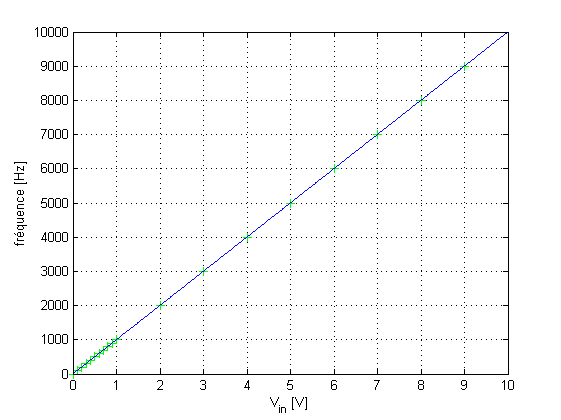
\includegraphics[scale=0.7]{img/vco_vs_reality.png}
%	\caption{ Théroie Vs. mesures}
%	\label{fig:theory_vs_mesure}
%\end{figure}
\end{document}